\documentclass[letterpaper,14pt]{extarticle}

%%%%%%%%%%%%%%%%%%%%%%%%%%%%%%%%%
% IMPORTS OF NECESSARY PACKAGES %
%%%%%%%%%%%%%%%%%%%%%%%%%%%%%%%%%
\usepackage{amsgen,amsmath,amstext,amsbsy,amsopn,amssymb,amsthm,stackengine,breqn}
\usepackage[usenames,dvipsnames,svgnames,table]{xcolor}
\usepackage{color,soul}
\usepackage{array, nicefrac, mathtools}
\usepackage[bottom]{footmisc} % To keep the footnote at the bottom even after putting answering environments.
\usepackage[colorlinks=true,linkcolor=blue,urlcolor=blue]{hyperref}
\usepackage{verbatim,booktabs,float,relsize,setspace,enumitem,pbox,cleveref,multicol,multirow,xifthen}
\usepackage[font=normalsize,skip=0pt, justification=centering]{caption, subcaption}
\usepackage{censor, textcomp, multido,bbding, tikz, mdframed, epsdice}
\usepackage{fancyvrb}
\usepackage{amsmath}
\usepackage{svg}

%%%%%%%%%%%%%%%%%%%%%%
% SOME COOL COMMANDS %
%%%%%%%%%%%%%%%%%%%%%%

% NULL character and SPACE symbol
\newcommand{\nullc}{\texttt{\textbackslash 0}}
\newcommand{\SPC}{\texttt{SPC}}

% Sets

\newcommand{\N}{\ensuremath{\mathbb{N}}}
\newcommand{\Z}{\ensuremath{\mathbb{Z}}}
\newcommand{\Q}{\ensuremath{\mathbb{Q}}}
\newcommand{\R}{\ensuremath{\mathbb{R}}}
\newcommand{\C}{\ensuremath{\mathbb{C}}}


\usepackage[inner=1cm,outer=1cm,top=1cm,bottom=2cm]{geometry}
\setlength{\parindent}{2em}
\setlength{\itemindent}{.5in}

%%%%%%%%%%%%%%%%%%%%%%%%%%%%%%%%%%%%%%%%%%%%%%%%%%%%%%%%%%%%%%%%%%%%%%%%%
%%%%%%%%%%%%%%%%%%%%%%%%%%%%%%%%%%%%%%%%%%%%%%%%%%%%%%%%%%%%%%%%%%%%%%%%%

% Matrix Code
%    $\left[\begin{array}{ccc}
%        0 & 0 & 1 \\
%        0 & 1 & 1 \\
%        1 & 1 & 1 \\
%   \end{array} \right]

% Table Code
% \begin{center}
% 	\begin{table}[H]
% 		\setlength{\tabcolsep}{10pt}
% 		\centering
% 		\renewcommand{\arraystretch}{1.0}
% 		\begin{tabular}{|c|c|c|} \hline 
% 			x & y & z \\ \hline
% 			a & b & c \\ \hline
% 		\end{tabular}
% 	\end{table}
% \end{center}

%%%%%%%%%%%%%%%%%%%%%%%%%%%%%%%%%%%%%%%%%%%%%%%%%%%%%%%%%%%%%%
%
%  BEGIN
%
%%%%%%%%%%%%%%%%%%%%%%%%%%%%%%%%%%%%%%%%%%%%%%%%%%%%%%%%%%%%%%
\begin{document}
\edef\tmp{\the\baselineskip}
\setstackgap{L}{\tmp}
$   $\newline
\underline{Formula Sheet 3}
\begin{itemize}
    \item Jean's Mass: $M_{critical} = 18M_\odot \sqrt{\frac{T^3}{\rho}}$
    \begin{itemize}
        \item $M_{critical}$ is the mass necessary for a cloud to condense.
        \item $M_\odot$ is the mass of the Sun, $\approx 2 \times 10^{30}\ kg$.
        \item $T$ is the temperature of the gas cloud, measured in Kelvin.
        \item $\rho$ is the density of the gas cloud, measured in $\frac{particles}{cm^2}$.
    \end{itemize}
    \item Scale Factor vs. Redshift: $\frac{a_{today}}{a_0} = 1 + z$
    \begin{itemize}
        \item $a_{today}$ is the scale factor today (usually set to 1).
        \item $a_0$ is the scale factor at the time the light was emitted.
        \item $z$ is the redshift observed.
    \end{itemize}
    \item Schwarzschild Radius: $r_{schwarzschild} = \frac{2GM}{c^2} \approx (3\ km) \frac{M}{M_\odot}$
    \begin{itemize}
        \item $r_{schwarzschild}$ is the radius of the event horizon if not distorted by any other factors.
        \item $G$ is the Universal Gravitational Constant, $6.67 \times 10^{-11}\ Nm^2kg^{-2}$ (number changes depending on units).
        \item $M$ is the mass of the black hole.
        \item $c$ is the speed of light, $3 \times 10^8\ \frac{m}{s}$. 
        \item $M_\odot$ is the mass of the Sun, $\approx 2 \times 10^{30}\ kg$.
    \end{itemize}
\end{itemize}
\pagebreak
\underline{Formula Sheet 2}
\begin{itemize}
    \item Absolute vs. Apparent Magnitude: $M = m - 5\log(d) + 5$ or $m = M + 5\log(d) - 5$
    \begin{itemize}
        \item $M$ is the absolute magnitude
        \item $m$ is the apparent magnitude
        \item $d$ is the distance from the object to the observer measured in parsecs.
        \item The logarithm is in base 10.
    \end{itemize}
    \item Absolute Magnitude vs. Luminosity: $\frac{L_1}{L_2} = 10^{\frac{2}{5}(M_2 - M_1)}$
        \begin{itemize}
        \item $L_1, L_2$ are the luminosities of object 1, object 2 respectively.
        \item $M_1, M_2$ are the absolute magnitudes of object 1, object 2 respectively.
        \item Note this is the exact same relation as Apparent Magnitude vs. Apparent Brightness.
    \end{itemize}
    \item Apparent Brightness (Inverse Square Law): $F = \frac{L}{4\pi r^2}$ 
    \begin{itemize}
        \item $F$ is apparent brightness (flux). See Stefan-Boltzmann Law for Power generated per $m^2$.
        \item $L$ is the object's luminosity.
        \item $r$ is the distance between the object and the observer.
    \end{itemize}
    \item Apparent Magnitude vs. Apparent Brightness: $\frac{F_1}{F_2} = 10^{\frac{2}{5}(m_2 - m_1)}$
    \begin{itemize}
        \item $F_1, F_2$ are the apparent brightnesses of object 1, object 2 respectively.
        \item $m_1, m_2$ are the apparent magnitudes of object 1, object 2 respectively.
        \item Note this is the exact same relation as Absolute Magnitude vs. Luminosity.
    \end{itemize}
    \item Change of Distance (Apparent Magnitude): $10^{\frac{2}{5}(m_1 - m_2)} = (\frac{d_1}{d_2})^2$ 
    \begin{itemize}
        \item $m_1$ is the initial magnitude.
        \item $m_2$ is the final magnitude.
        \item $d_1$ is the initial distance. If $d_2 = 10\ pc$, $m_2$ is absolute magnitude, then
        \newline 
        $d_1 = 10^{\frac{m - M + 5}{5}}$
        \item $d_2$ is the final distance. If final distance is $10\ pc$, simplifies to Absolute vs. Apparent Magnitude equation.
    \end{itemize}
    \pagebreak
    \item Radius vs. Luminosity and Temperature: $\frac{R_1}{R_2} = (\frac{T_2}{T_1})^2 \sqrt{\frac{L_1}{L_2}}$
    \begin{itemize}
        \item $R_1, R_2$ are the radii of object 1, object 2 respectively.
        \item $T_1, T_2$ are the surface temperatures of object 1, object 2 respectively.
        \item $L_1, L_2$ are the luminosities of object 1, object 2 respectively.
    \end{itemize}
    \item Relativistic Length Contraction: $L_{obs} = \frac{L_{prop}}{\gamma}$
    \begin{itemize}
        \item $L_{obs}$ is the length measured by an observer moving relativistically.
        \item $L_{prop}$ is the length measured at rest.
        \item $\gamma$ is the Lorentz Factor: $\frac{1}{\sqrt{1 - \frac{v^2}{c^2}}}$
    \end{itemize}
    \item Relativistic Mass Multiplication: $m_{obs} = m_{prop}\gamma$
    \begin{itemize}
        \item $m_{obs}$ is the mass measured by an observer moving relativistically.
        \item $m_{prop}$ is the mass measured at rest.
        \item $\gamma$ is the Lorentz Factor: $\frac{1}{\sqrt{1 - \frac{v^2}{c^2}}}$
    \end{itemize}
    \item Relativistic Time Dilation: $t_{obs} = t_{prop}\gamma$
    \begin{itemize}
        \item $t_{obs}$ is the time measured by an observer moving relativistically.
        \item $t_{prop}$ is the time measured at rest.
        \item $\gamma$ is the Lorentz Factor: $\frac{1}{\sqrt{1 - \frac{v^2}{c^2}}}$
    \end{itemize}
    \item Relativistic Velocity Addition: $v = \frac{v_1 + v_2}{1 + \frac{v_1v_2}{c^2}}$
    \begin{itemize}
        \item $v$ is the final velocity.
        \item $v_1$ is the velocity of object 1.
        \item $v_2$ is the velocity of object 2.
        \item $c$ is the speed of light, $3 \times 10^8\ \frac{m}{s}$.
    \end{itemize}
    \item (Heisenberg's) Uncertainty Principle: $\Delta x \Delta p \geq \frac{h}{4\pi}$
    \begin{itemize}
        \item $\Delta x$ is the uncertainty in position.
        \item $\Delta p$ is the uncertainty in momentum.
        \item $h$ is Planck's constant, for Joules and seconds, $6.63 \times 10^{-34}\ Js$.
    \end{itemize}
\end{itemize}
\pagebreak
\underline{Formula Sheet 1}
\begin{itemize}
    \item Angular Momentum (circular motion, in $\frac{kgm^2}{s}$): $L = rmv_{\perp}$
    \begin{itemize}
        \item $L$ is the angular momentum.
        \item $r$ is the radius of the circle.
        \item $m$ is the mass of the moving object.
        \item $v_{\perp}$ is the perpendicular component of velocity.
    \end{itemize}
    \item Angular Resolution / Diffraction Limit (in arcseconds): $L = 2.5 \times 10^5 \frac{\lambda}{d_{\text{telescope}}}$
    \begin{itemize}
        \item $L$ is the diffraction limit.
        \item $\lambda$ is the wavelength of light targeted.
        \item $d_{\text{telescope}}$ is the diameter of the telescope.
    \end{itemize}
    \item Angular Size / Angular Separation (in degrees): $\theta = d_{\text{actual}} \times \frac{360^\circ}{2\pi d_{\text{to Earth}}}$
    \begin{itemize}
        \item $d_{\text{actual}}$ is the diameter of object (size) or the distance between the two objects (separation)
        \item $d_{\text{to Earth}}$ is the distance between the object and Earth.
    \end{itemize}
    \item Arc Length (same units as radius): $s = \theta r$
    \begin{itemize}
        \item $s$ is the arc length.
        \item $\theta$ is the angle swept by the arc, in radians. If in degrees, use $\frac{\theta\pi}{180}$.
        \item $r$ is the radius (or radial distance) of the object.
        \item Notable use case is Eratosthenes' circumference of Earth approximation with known $\theta$ and $s$ as well as approximating actual diameter of a far away object given angular size and distance from Earth.
    \end{itemize}
    \item Center of Mass (of two bodies): $\frac{m_1d_1 + m_2d_2}{m_1 + m_2}$
    \begin{itemize}
        \item $m_1, m_2$ are the masses of the two objects.
        \item $d_1, d_2$ are the distances of the two objects.
    \end{itemize}
    \pagebreak
    \item Doppler Effect: $\frac{\lambda_{\text{observed}} - \lambda_{\text{actual}}}{\lambda_{\text{actual}}} = \frac{v_{\text{rad}}}{c}$
    \begin{itemize}
        \item $\lambda_{\text{observed}}$ is wavelength observed from the object.
        \item $\lambda_{\text{actual}}$ is the wavelength that the object actually emits (found from measurements on Earth).
        \item $v_{\text{rad}}$ is the radial component (the component moving towards or away from us).
        \item $c$ is the speed of light, $3 \times 10^8\ \frac{m}{s}$
    \end{itemize}
    \item Ellipse Eccentricity: $e = \sqrt{1 - \frac{b^2}{a^2}} = \frac{c}{a}$
    \begin{center}
    % Figure licensed under creative commons by Ag2gaeh - https://en.wikipedia.org/wiki/File:Ellipse-def0.svg
        \includesvg[scale=1.5]{ellipse.svg}
    \end{center}
    \begin{itemize}
        \item $e$ is the eccentricity of the object.
        \item $a$ is the length of the semi-major axis (think of it as the longer radius).
        \item $b$ is the length of the semi-minor axis (think of it as the shorter radius).
        \item $c$ is the distance from the center to a focus. Can be calculated with $c = ae$
    \end{itemize}
    \pagebreak
    \item Energy: $E_{\text{total}} = KE + PE$
    \begin{itemize}
        \item $E_{\text{total}}$ is the total energy of the object.
        \item $KE$ is the kinetic energy of the object, calculated with $KE = \frac{1}{2}mv^2$
        \begin{itemize}
            \item $m$ is the mass of the object.
            \item $v$ is the velocity of the object.
        \end{itemize}
        \item $PE$ is the potential energy of the object, usually gravitational potential energy. Can be calculated with $PE = -\frac{GM_1M_2}{r}$ or on the surface of Earth, $mgh$.
        \begin{itemize}
            \item $G$ is the Universal Gravitational Constant, $6.67 \times 10^{-11}\ Nm^2kg^{-2}$ (number changes depending on units).
            \item $M_1, M_2$ are the mass of the two bodies.
            \item $r$ is the distance between the two bodies.
            \item $m$ is the mass of the object on Earth.
            \item $g$ is the acceleration due gravity on Earth, $g \approx -9.8 \frac{m}{s^2}$.
            \item $h$ is the height of the object from the surface.
        \end{itemize}
    \end{itemize}
    \item Escape Velocity (usually in $\frac{m}{s}$ or $\frac{km}{s}$): $v_{esc} = \sqrt{\frac{2GM}{R}}$
    \begin{itemize}
        \item $v_{esc}$ is the velocity needed to escape from the orbit of a body.
        \item $G$ is the Universal Gravitational Constant, $6.67 \times 10^{-11}\ Nm^2kg^{-2}$ (number changes depending on units).
        \item $M$ is the mass of the object you're escaping from.
        \item $R$ is your distance from the center of the object.
    \end{itemize}
    \item Kepler's Third Law: $P^2 \propto a^3$; Newton's Version: $P^2 = \frac{4\pi^2}{G(M_1 + M_2)}a^3$
    \begin{itemize}
        \item $P$ is the orbital period (measure of time)
        \item $a$ is the semi-major axis of the orbit (measure of distance)
        \item $G$ is the Universal Gravitational Constant, $6.67 \times 10^{-11}\ Nm^2kg^{-2}$ (number changes depending on units).
        \item $M_1, M_2$ are the masses of the objects, usually one is a star and the other is a planet (but not necessarily). Newton's version can be re-arranged to solve for mass: $M_1 + M_2 = \frac{4\pi^2}{GP^2}a^3$.
    \end{itemize}
    \pagebreak
    \item Law of Universal Gravitation (in $N$): $F_g = \frac{GM_1M_2}{r^2}$
    \begin{itemize}
        \item $F_g$ is the force of gravity that the objects exert on each other.
        \item $G$ is the Universal Gravitational Constant, $6.67 \times 10^{-11}\ Nm^2kg^{-2}$ (number changes depending on units).
        \item $M_1, M_2$ are the masses of the two objects.
        \item $r$ is the distance between the two objects.
    \end{itemize}
    \item Mass-Energy Equivalence (usually in $J$): $E = mc^2$
    \begin{itemize}
        \item $E$ is the energy associated with the mass.
        \item $m$ is the mass being converted into energy.
        \item $c$ is the speed of light, $3 \times 10^8\ \frac{m}{s}$.
    \end{itemize}
    \item Momentum (in $\frac{kgm}{s} or Ns$): $p = mv$
    \begin{itemize}
        \item $p$ is the momentum.
        \item $m$ is the mass of the object.
        \item $v$ is the velocity of the object.
        \item Useful context: calculating conservation of momentum (set initial and final momentum equal to each other and solve for a variable).
    \end{itemize}
    \item Motion: $x, s, v, a$ and $t$
    \begin{itemize}
        \item $x$ is the displacement of the object (has both magnitude and direction).
        \item $s$ is the speed of the object, calculated with $s = \frac{\|\Delta x\|}{\Delta t}$. Does not have direction.
        \item $v$ is the velocity of the object (has both magnitude and direction). Calculated with $v = \frac{\Delta x}{\Delta t}$.
        \item $a$ is the acceleration of the object (has both magnitude and direction). Calculated with $a = \frac{\Delta v}{\Delta t}$
        \item $t$ is time, $\Delta t$ is the change in time.
    \end{itemize}
    \item Newton's Second Law (in $N$): $F = ma = \frac{dp}{dt}$
    \begin{itemize}
        \item $F$ is the net force exerted on the object.
        \item $m$ is the mass of the object.
        \item $a$ is the acceleration associated with the net force.
        \item $\frac{dp}{dt}$ is the derivative of momentum with respect to time. Think of it as the change in momentum over time. When $F = 0$, momentum is constant.
    \end{itemize}
    \item Stefan-Boltzmann Law: Power per Square Meter = $\sigma T^4$
    \begin{itemize}
        \item $\sigma$ is the Stefan-Boltzmann Constant, $5.7 \times 10^{-8}\ Wm^{-2}K^{-4}$
        \item $T$ is the temperature of the object, in Kelvin.
    \end{itemize}
    \item Stellar Parallax: $d_{\text{to object}} = \frac{r}{p}$
    \begin{center}
    % Figure in public domain - https://commons.wikimedia.org/wiki/File:Stellarparallax_parsec1.svg
        \includesvg[scale=0.6]{parallax.svg}
    \end{center}
    \begin{itemize}
        \item $d_{\text{to object}}$ is the distance from the Earth to the observed body.
        \item $r$ is the amount of distance the observer moves in order to observe parallax. In the context of Earth, this is $1\ AU = 1.5 \times 10^{11}\ m$.
        \item $p$ is the parallax angle, or the angle the surroundings change at.
    \end{itemize}
    \item Torque (in $Nm$): $\tau = F_{\perp}r$
    \begin{itemize}
        \item $\tau$ is Torque.
        \item $F_{\perp}$ is the perpendicular component of the Force.
        \item $r$ is the radius of the circular motion.
    \end{itemize}
    \item (Electromagnetic) Wave Properties: $\lambda f = c$, $E = hf$
    \begin{itemize}
        \item $\lambda$ is the wavelength of the wave. Can be calculated with $\lambda = \frac{c}{f}$.
        \item $f$ is the frequency of the wave. Can be calculated with $f = \frac{c}{\lambda}$.
        \item $c$ is the speed of light, $3 \times 10^8\ \frac{m}{s}$.
        \item $E$ is the energy of the wave.
        \item $h$ is Planck's constant, for Joules and seconds, $6.63 \times 10^{-34}\ Js$.
    \end{itemize}
    \item Wien's Law: $\lambda_{\text{peak}} = \frac{b}{T}$
    \begin{itemize}
        \item $\lambda_{\text{peak}}$ is the wavelength that the object radiates with highest relative intensity.
        \item $b$ is Wien's Displacement Constant, equal to $2.9 \times 10^{-3}\ mK$ or $2.9 \times 10^6\ nmK$
        \item $T$ is the temperature of the object.
    \end{itemize}
\end{itemize}
\pagebreak
\underline{Additonal Useful Info}
\begin{itemize}
    \item Luminosity Classes
    \begin{itemize}
        \item Give information about the star's radius.
        \item I - Supergiant
        \item II - Bright Giant
        \item III - Giant
        \item IV - Subgiant
        \item V - Main Sequence Star
        \item VI, VII - Subdwarf, White Dwarf
    \end{itemize}
    \item Spectral Types
    \begin{itemize}
        \item Give information about the star's surface temperature. In order of hottest to coolest:
        \item O, B, A, F, G, A, K, M
        \item Types also have subclasses numbered 0-9. Within each class, 0 subclass stars are hottest and 9 subclass stars are the coolest. For example, B0 is hotter than B1, but A0 is cooler than B9.
    \end{itemize}
    \item Spacetime Diagrams
    \begin{itemize}
        \item Tell you how a an object moves through spacetime.
        \item x-axis is position, y-axis is time. Usually in light seconds and seconds as their respective units.
        \item Stationary objects will be a vertical line, objects at a constant velocity move in a straight line, and accelerating objects will move in a curved line.
        \item Light is usually a $45^\circ$ line or $-45^\circ$. Any slope less than that is impossible (moving faster than light).
        \begin{center}
        % Graphic made by me. Feel free to do whatever you want with it. I waive all rights to it.
            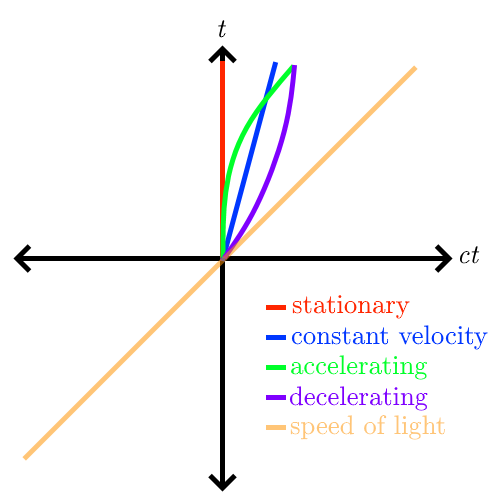
\includegraphics[scale=0.5]{std-fig.png}
        \end{center}
    \end{itemize}
    \item Stellar Classification
    \begin{itemize}
        \item Brown Dwarfs: $\leq 0.08M_\odot$. Not really stars (degeneracy pressure prevents fusion)
        \item Low-Mass Stars: $0.08M_\odot < M \leq 2M_\odot$.
        \item Intermediate Mass Stars: $2M_\odot < M \leq 8 M_\odot$.
        \item High Mass Stars: $> 8M_\odot$.
        \item Upper limit: $\approx 150M_\odot$.
    \end{itemize}
    \item Hubble's Law: Galaxies are moving away from us at $H_0 \approx 70 \frac{km/s}{pc}$.
    \begin{itemize}
        \item Find the distance an object is at given velocity $v$ with $d = \frac{v}{H_0}$
        \item Find the age of the universe with $H(t)^{-1} \approx 13.8\ Ga$.
    \end{itemize}
    \item Distance Ladder
    \begin{itemize}
        \item Find the closest objects using radio technologies.
        \item Find the distance of items within parsecs using Stellar Parallax.
        \item Find the distance of further objects using Cepheids as a standard candle.
        \item The furthest objects are found using Supernova Type Ia (white dwarf supernovae) as a standard candle.
    \end{itemize}
    \pagebreak
    \item H-R Diagrams
    \begin{itemize}
        \item Plots the temperature and spectral class on the horizontal axis. Hotter stars are further to the left.
        \item Plots the luminosity on the vertical axis. More luminous stars are higher.
        \item Main sequence stars that fuse hydrogen are all generally shown on a diagonal line.
        \item Protostars and giant stars are to the top and right of their respective main sequence stars.
    \end{itemize}
    \begin{center}
    % Figure provided by ESO under Creative Commons licensing - https://www.eso.org/public/images/eso0728c/
        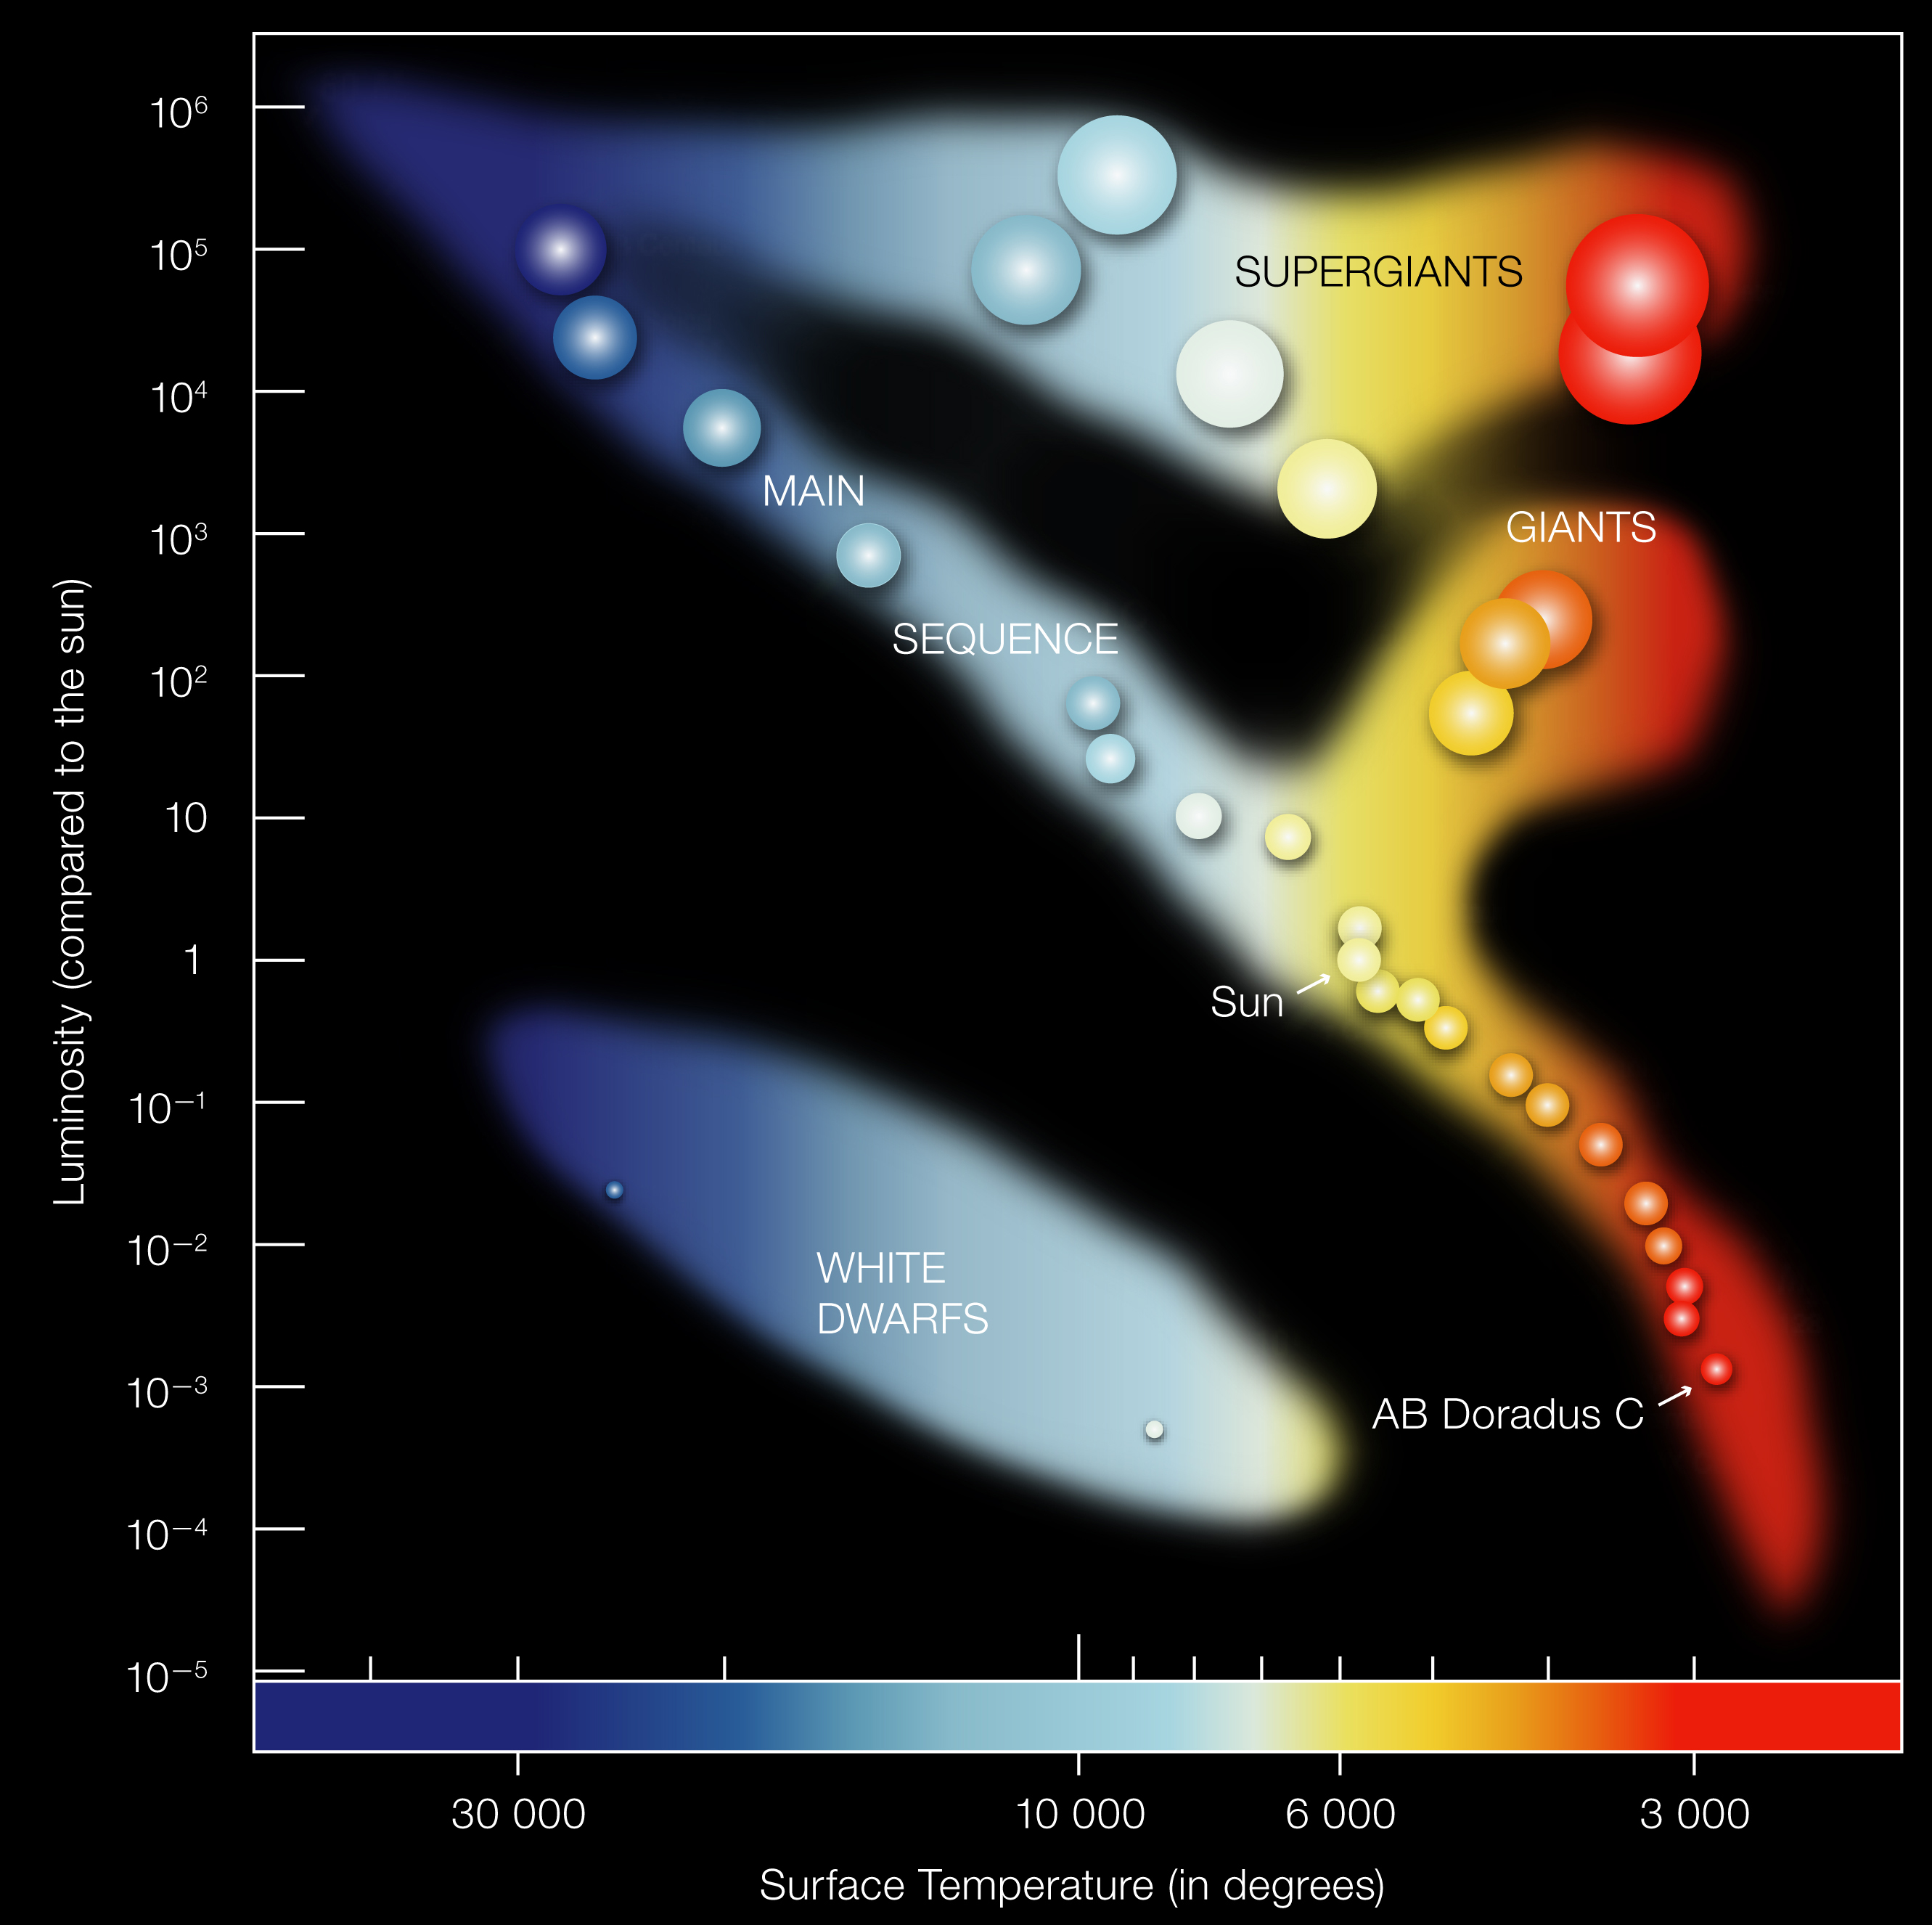
\includegraphics[scale=0.7]{hr.png}
    \end{center}
\end{itemize}
\end{document}